\documentclass[convert]{standalone}

\usepackage{tikz}
\usepackage{graphicx}
\pagestyle{empty}

% INT_AY22_L28-Fig02_Pulse_Faraday_law.png

\begin{document}
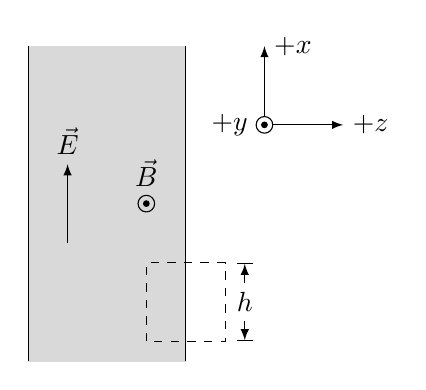
\begin{tikzpicture}[> = latex]

	% EM pulse region
	
	\filldraw [gray!30] (-1, -2) rectangle (1, 2);
	\draw (-1, -2) -- (-1, 2);
	\draw (1, -2) -- (1, 2);
	
	% Field directions inside region
	
	\draw [->] (-0.5, -0.5) -- (-0.5, 0.5) node [above] {${\vec E}$};
	
	\draw (0.5, 0) circle (3 pt) node [above = 0.25 em] {${\vec B}$};
	\filldraw (0.5, 0) circle (1 pt);
	
	% Coordinate axes
	
	\draw [->] (2, 1) -- (3, 1) node [right] {$+z$};
	\draw [->] (2, 1) -- (2, 2) node [right] {$+x$};
	
	\draw [fill = white] (2, 1) circle (3 pt) node [left = 0.25 em] {$+y$};
	\filldraw (2, 1) circle (1 pt);
	
	% Amperian loop w labels
	
	\draw [dashed] (0.5, -1.75) -- (0.5, -0.75) -- (1.5, -0.75) -- (1.5, -1.75) -- cycle;
	\draw [|<->|] (1.75, -1.75) -- node [fill = white] {$h$} (1.75, -0.75);

\end{tikzpicture}
\end{document}